\documentclass[10pt,a4paper]{article}

\usepackage[utf8]{inputenc}
\usepackage[T5]{fontenc}
\usepackage[vietnamese,english]{babel}
\usepackage{lmodern}
\usepackage{microtype}
\usepackage{geometry}
\usepackage{amsmath,amssymb}
\usepackage{graphicx}
\usepackage{booktabs}
\usepackage{tabularx}
\usepackage{array}
\usepackage{multirow}
\usepackage{caption}
\usepackage{subcaption}
\usepackage[section]{placeins}
\usepackage{xcolor}
\usepackage{enumitem}
\usepackage{xurl}
\usepackage{hyperref}
\usepackage{fancyhdr}

\geometry{top=2.0cm,bottom=2.1cm,left=2.05cm,right=2.05cm}
\setlength{\parindent}{1.1cm}
\setlength{\parskip}{0.15em}
\setlist{nosep,leftmargin=1.6em}
\captionsetup{font=small,labelfont=bf}
\renewcommand{\arraystretch}{1.13}
\newcolumntype{Y}{>{\raggedright\arraybackslash}X}
\newcolumntype{C}[1]{>{\centering\arraybackslash}p{#1}}

\definecolor{linkblue}{RGB}{18,82,148}
\hypersetup{
  colorlinks=true,
  linkcolor=linkblue,
  citecolor=linkblue,
  urlcolor=linkblue,
  pdftitle={Lựa chọn kiến trúc và tiền xử lý khi chuyển bộ dữ liệu trong phân giai đoạn giấc ngủ từ EEG đơn kênh: Đánh giá có kiểm soát trên Sleep-EDF và SHHS1},
  pdfauthor={Ngô Nhật Quân; Phạm Thái Sơn}
}

\pagestyle{fancy}
\fancyhf{}
\fancyhead[L]{Lựa chọn pipeline và chuyển miền trong phân giai đoạn giấc ngủ}
\fancyhead[R]{Bản thảo nghiên cứu}
\fancyfoot[C]{\thepage}
\setlength{\headheight}{13pt}

\newcommand{\mf}{\ensuremath{\mathrm{Macro\mbox{-}F1}}}
\newcommand{\ci}{\ensuremath{\mathrm{CI}_{95\%}}}

\title{\textbf{Lựa chọn kiến trúc và tiền xử lý khi chuyển bộ dữ liệu trong phân giai đoạn giấc ngủ từ EEG đơn kênh: Đánh giá có kiểm soát trên Sleep-EDF và SHHS1}\\[0.55em]
\large Architecture and Preprocessing Choices under Dataset Shift in Single-Channel EEG Sleep Staging: A Controlled Evaluation on Sleep-EDF and SHHS1}
\author{Ngô Nhật Quân\thanks{Tác giả chính và tác giả liên hệ: \texttt{23521258@gm.uit.edu.vn}} \and Phạm Thái Sơn\\
\small Trường Đại học Công nghệ Thông tin, Đại học Quốc gia TP. Hồ Chí Minh\\
\small Khu phố 34, phường Linh Xuân, Thành phố Hồ Chí Minh, Việt Nam}
\date{Bản thảo nghiên cứu, tháng 9 năm 2026}

\begin{document}
\renewcommand{\refname}{Tài liệu tham khảo}
\maketitle

\renewcommand{\abstractname}{Tóm tắt}
\begin{abstract}
Nghiên cứu so sánh sáu cấu hình phân giai đoạn giấc ngủ từ EEG đơn kênh trên cùng phép chia theo 78 đối tượng Sleep-EDF Expanded và đánh giá chuyển sang SHHS1. Các đối chiếu phân biệt thay cấu hình mô hình chuỗi, thay gói đặc trưng/ngữ cảnh và thay tiền xử lý; khác biệt về lịch huấn luyện được khai báo riêng. ResNet-1D--TCN với chế độ xử lý biên độ cố định E3 đạt \mf\ ngoài fold 0,7904, cao nhất ở seed 42. E3 cao hơn E6 0,0213 (\ci\ $[0,0122;0,0307]$, $p_{Holm}=0,0012$); lần lặp seed 123 giữ chênh lệch gộp dương nhưng không đạt ý nghĩa Wilcoxon sau Holm. E6 dùng trung bình và độ lệch chuẩn của toàn bộ bản ghi đích không nhãn nên có tính transductive ở cấp bản ghi. ResNet-1D--TCN suy luận nhanh hơn E0 khoảng 3,76 lần trong benchmark, đổi lại số tham số cao hơn 4,37 lần và bộ nhớ GPU cực đại cao hơn 28,4\%. Trên 180 đối tượng SHHS1 đã khóa, E3 cao hơn E0 và E6 theo \mf\ trung bình ở cấp đối tượng, nhưng E0/E3 đều gán hơn 72\% epoch N3 thành N2, với recall N3 lần lượt 0,2610/0,2582. E6 cũng không khắc phục thiếu hụt này. Đóng góp nằm ở lợi ích tổng thể, đánh đổi vận hành được định lượng và lỗi N3 tái diễn qua các pipeline, thay vì một ưu thế kiến trúc riêng lẻ hoặc biện pháp thích nghi đã được kiểm chứng.
\end{abstract}

\noindent\textbf{Từ khóa:} phân giai đoạn giấc ngủ; EEG đơn kênh; mạng tích chập thời gian; tiền xử lý; dịch chuyển miền; đánh giá bắt cặp.

\begin{center}
\rule{0.95\textwidth}{0.35pt}
\end{center}

\selectlanguage{english}
\renewcommand{\abstractname}{Abstract}
\begin{abstract}
We evaluated six single-channel EEG sleep-staging configurations under shared subject partitions on 78 Sleep-EDF Expanded participants and assessed transfer to SHHS1. The comparisons distinguished sequence-model configurations, feature/context packages and preprocessing, with their training settings reported explicitly. The fixed-scale ResNet-1D--TCN configuration E3 achieved the highest seed-42 out-of-fold macro-F1 (0.7904), exceeding E6 by 0.0213 (95\% CI $[0.0122,0.0307]$, Holm-adjusted $p=0.0012$). The seed-123 sensitivity run retained a positive pooled difference but not Holm significance in the subject-level Wilcoxon analysis. E6 estimates normalization statistics from each complete unlabelled target recording and therefore has a transductive dependency. E3 provided a 3.76-fold inference speed-up over E0 in the benchmark, at the cost of 4.37 times more parameters and 28.4\% higher peak GPU memory. On 180 locked SHHS1 participants, E3 exceeded E0 and E6 in subject-mean macro-F1. Nevertheless, E0 and E3 each misclassified more than 72\% of N3 epochs as N2, with N3 recall of 0.2610 and 0.2582; E6 did not remedy this deficit. The results quantify pipeline-level performance and operational trade-offs while identifying a recurring N3 transfer error, without establishing an architecture-only advantage or a validated adaptation remedy.
\end{abstract}
\noindent\textbf{Keywords:} sleep staging; single-channel EEG; temporal convolutional network; preprocessing; domain shift; paired evaluation.
\selectlanguage{vietnamese}

\section{Giới thiệu}

Phân giai đoạn giấc ngủ gán một trong năm nhãn W, N1, N2, N3 và REM cho mỗi epoch 30 giây của bản ghi đa ký giấc ngủ. Công việc thủ công tốn thời gian, cần chuyên môn và vẫn có bất đồng giữa người chấm; chương trình độ tin cậy liên chấm của AASM cho thấy N1 có mức đồng thuận thấp nhất~\cite{rosenberg2013aasm}. Do đó, một hệ thống tự động không chỉ cần độ chính xác tổng thể mà còn phải được đánh giá bằng chỉ số cân bằng lớp, tính ổn định theo người và khả năng tổng quát sang thiết bị hoặc quần thể khác.

ZleepAnlystNet là mô hình EEG đơn kênh hai giai đoạn, kết hợp bộ trích đặc trưng CNN với BiLSTM~\cite{jadhav2024zleepanlystnet}. Nghiên cứu khảo sát TCN như một mô hình chuỗi có khả năng xử lý song song~\cite{bai2018tcn} và ResNet-1D như một bộ trích đặc trưng có kết nối dư~\cite{he2016resnet}. Các lựa chọn này có thể đem lại lợi ích vận hành hoặc biểu diễn, nhưng không mặc nhiên bảo đảm chất lượng dự đoán cao hơn. Chế độ xử lý biên độ cũng được xem xét vì có thể ảnh hưởng đáng kể khi chuyển giữa các thiết bị và quần thể.

Nghiên cứu thiết kế một chiến dịch bắt cặp theo đối tượng để trả lời bốn câu hỏi: (1) thay cấu hình BiLSTM bằng cấu hình TCN, cùng lịch huấn luyện tương ứng nhưng giữ encoder, có đem lại lợi ích hay không; (2) thay gói đặc trưng/ngữ cảnh C/P/N 75 chiều của E1 bằng encoder ResNet-1D 128 chiều chỉ dùng epoch hiện tại có tạo lợi ích hay không; (3) các chế độ tiền xử lý cho kết quả khác nhau thế nào; và (4) thứ hạng cùng cấu trúc sai số thay đổi ra sao khi chuyển sang SHHS1.

Đóng góp chính là bằng chứng bắt cặp về hiệu năng và đánh đổi vận hành của các cấu hình pipeline, cùng phân tích lỗi ngoài miền tái diễn qua hai họ mô hình. Phép chia 10-fold theo đối tượng và cơ chế khóa test bảo vệ tính hợp lệ của các đối chiếu; phân tích không gian đặc trưng và loại bỏ ngữ cảnh cung cấp bằng chứng hỗ trợ. Nghiên cứu phân biệt so sánh được nêu trong giao thức, phân tích thứ cấp và phân tích hậu nghiệm, không coi mọi thay đổi pipeline là phép cô lập một thành phần.

\section{Nghiên cứu liên quan}

DeepSleepNet kết hợp CNN hai nhánh và BiLSTM để học hình thái epoch cùng quan hệ theo thời gian~\cite{supratak2017deepsleepnet}. AttnSleep sử dụng cơ chế chú ý và mô hình hóa thời gian~\cite{eldele2021attnsleep}; SleepTransformer khai thác self-attention và ước lượng bất định~\cite{phan2022sleeptransformer}. Các công trình này cho thấy ngữ cảnh chuỗi quan trọng, nhưng khác biệt về tập dữ liệu, phép chia và tiền xử lý khiến việc so sánh chéo bảng không thay thế được ablation trong cùng giao thức.

SleepInceptionNet khảo sát có hệ thống tín hiệu thô, phổ và biểu diễn thời gian--tần số, sau đó chọn một mô hình Inception dùng biến đổi wavelet liên tục trên EEG trung tâm đơn kênh để chấm từng epoch~\cite{haghayegh2023sleepinceptionnet}. Công trình này cho thấy lựa chọn biểu diễn đầu vào là một phần của định nghĩa pipeline, không phải chi tiết triển khai trung tính. Ở hướng chuyển miền, ADAST dùng attention riêng theo miền, căn chỉnh đối kháng và self-training bằng pseudo-label từ dữ liệu đích không nhãn~\cite{eldele2023adast}. Khác với ADAST, E6 trong nghiên cứu hiện tại chỉ dùng thống kê chuẩn hóa của bản ghi đích và không cập nhật biểu diễn hoặc trọng số mô hình.

Sleep-EDF Expanded là mốc phổ biến cho EEG đơn kênh~\cite{kemp2000sleepEDF,physionetSleepEDF}. SHHS là nghiên cứu đoàn hệ đa trung tâm quy mô lớn, được thu thập để nghiên cứu rối loạn hô hấp khi ngủ và nguy cơ tim mạch~\cite{quan1997shhs}; dữ liệu được phân phối qua National Sleep Research Resource (NSRR)~\cite{zhang2018nsrr}. Khác biệt giữa Sleep-EDF và SHHS về tuổi, bệnh lý, thiết bị, montage và phân bố nhãn tạo ra phép kiểm tra dịch chuyển miền thực tế hơn đánh giá trong cùng bộ dữ liệu.

Davidson và cộng sự khảo sát tiêu chí chấm N3 trên 2.913 bản ghi SHHS, nhấn mạnh mối liên hệ giữa ngưỡng sóng chậm, tuổi và giới trong kết quả chấm~\cite{davidson2025n3}. Bối cảnh này giúp đặt lỗi N3 ngoài miền vào một vấn đề đã được nghiên cứu, nhưng không chứng minh nguyên nhân lỗi của các pipeline hiện tại. Điểm tập trung của nghiên cứu là kết hợp so sánh cấu hình bắt cặp, đánh đổi vận hành và sai số theo lớp khi chuyển cohort; không xếp hạng trực tiếp với các công trình dùng dữ liệu hoặc giao thức khác.

\section{Vật liệu và phương pháp}

\subsection{Dữ liệu và nhãn}

Sleep-EDF Expanded Sleep Cassette gồm 153 bản ghi của 78 đối tượng, sử dụng kênh Fpz--Cz. Nhãn được ánh xạ về W, N1, N2, N3 và REM; các epoch không hợp lệ được giữ đúng vị trí chuỗi nhưng không tham gia huấn luyện hoặc tính chỉ số. Sau cắt cửa sổ, có 195.469 epoch hợp lệ. Phân bố lớp được trình bày trong Bảng~\ref{tab:class-distribution}.

Mẫu SHHS Visit 1 gồm 180 đối tượng test trong danh sách đã khóa. Quy trình chọn dùng trường chất lượng \texttt{overall\_shhs1} với các giá trị hợp lệ 3--7 và thứ tự xác định bằng SHA-256 với selection seed 42, không dùng điểm số mô hình để chọn người. Tổng cộng 220 người được phân vào các vai trò: 5 adaptation, 15 validation, 180 test và 20 dự phòng; kiểm tra kỹ thuật ban đầu dùng 5 người adaptation và 5 người validation. Nghiên cứu không cập nhật trọng số bằng SHHS và không sử dụng nhóm dự phòng để thay người trong kết quả báo cáo. Tín hiệu C4--A1 được lấy mẫu lại từ 125 về 100 Hz. Dữ liệu SHHS chịu điều kiện truy cập NSRR; báo cáo không công bố mã định danh người tham gia.

\begin{table}[t]
\centering
\caption{Phân bố nhãn hợp lệ trong hai mẫu đánh giá.}
\label{tab:class-distribution}
\small
\begin{tabular}{lrr|rr}
\toprule
\textbf{Nhãn} & \multicolumn{2}{c|}{\textbf{Sleep-EDF}} & \multicolumn{2}{c}{\textbf{SHHS1 test}} \\
 & \textbf{Số epoch} & \textbf{Tỷ lệ} & \textbf{Số epoch} & \textbf{Tỷ lệ} \\
\midrule
W & 65.941 & 33,73\% & 36.983 & 21,88\% \\
N1 & 21.522 & 11,01\% & 7.002 & 4,14\% \\
N2 & 69.132 & 35,37\% & 76.287 & 45,14\% \\
N3 & 13.039 & 6,67\% & 22.806 & 13,49\% \\
REM & 25.835 & 13,22\% & 25.934 & 15,34\% \\
\midrule
\textbf{Tổng hợp lệ} & \textbf{195.469} & \textbf{100\%} & \textbf{169.012} & \textbf{100\%} \\
\bottomrule
\end{tabular}
\end{table}

Sleep-EDF còn 298 epoch Movement hoặc Unknown không tham gia chỉ số. Sự khác biệt phân bố, đặc biệt tỷ trọng N1 thấp hơn và N2 cao hơn trong SHHS1, được xem là một đặc điểm của mẫu ngoài miền chứ không phải hiệu ứng của mô hình.

\subsection{Tiền xử lý}

Tín hiệu được chuyển về $\mu\mathrm{V}$, căn chỉnh với nhãn và xử lý trên toàn bản ghi trước khi chia epoch. Lọc dải Butterworth bậc 4, 0,5--30 Hz, dùng thao tác tiến--lùi không lệch pha. E3 tiếp tục giới hạn ở $\pm800~\mu\mathrm{V}$ rồi chia 100; E4 chỉ lọc dải; E6 dùng cùng bước lọc và giới hạn nhưng thay phép chia 100 bằng z-score. Trung bình và độ lệch chuẩn E6 được tính trên toàn bộ tín hiệu sau lọc/giới hạn, trước khi cắt cửa sổ ngủ, kể cả phần ngoài cửa sổ đánh giá. Thống kê này không dùng nhãn hay dữ liệu gộp của cohort; ở miền đích, E6 vì vậy có tính transductive cấp bản ghi. Bản ghi có độ lệch chuẩn bằng 0 hoặc không hữu hạn bị từ chối, không được tự thay bằng một hằng số. E5 (lọc dải và giới hạn, không đổi thang) giống E4 từng bit trên 153/153 bản ghi Sleep-EDF nên không tạo điều kiện đầu vào độc lập.

Cửa sổ đánh giá giữ tối đa 30 phút Wake trước epoch ngủ đầu và sau epoch ngủ cuối, được xác định từ nhãn tham chiếu N1--N3/REM. Các epoch Movement/Unknown nằm bên trong được giữ vị trí và loại khỏi loss/chỉ số. Quy tắc cắt này dùng nhãn cho việc dựng mẫu đánh giá; nó không phải một bộ xác định cửa sổ triển khai không nhãn. Lọc không lệch pha, BiLSTM hai chiều và TCN không nhân quả đều phù hợp với phân tích ngoại tuyến.

\subsection{Cấu hình mô hình}

\begin{table}[t]
\centering
\caption{Các cấu hình được so sánh.}
\label{tab:configs}
\small
\begin{tabularx}{\textwidth}{lYYY}
\toprule
\textbf{Mã} & \textbf{Dữ liệu} & \textbf{Bộ trích xuất} & \textbf{Mô hình chuỗi và mục đích} \\
\midrule
E0 & Tín hiệu thô & CNN đối chứng & BiLSTM; đối chứng nội bộ \\
E1 & Tín hiệu thô & CNN đối chứng & TCN và lịch huấn luyện tương ứng; giữ encoder/đặc trưng E0 \\
E2 & Tín hiệu thô & ResNet-1D & TCN; thay gói đặc trưng/ngữ cảnh E1 bằng encoder epoch hiện tại \\
E3 & Lọc, giới hạn, chia 100 & ResNet-1D & TCN; pipeline xử lý biên độ cố định \\
E4 & Chỉ lọc dải & ResNet-1D & TCN; đối chiếu chế độ lọc dải \\
E6 & Lọc, cắt, z-score & ResNet-1D & TCN; đối chiếu cách đổi thang \\
\bottomrule
\end{tabularx}
\end{table}

E0 tái triển khai cấu trúc CNN--BiLSTM của ZleepAnlystNet làm đối chứng nội bộ. E1 dùng lại encoder và cache đặc trưng E0, thay BiLSTM bằng TCN cùng các thiết lập huấn luyện tương ứng; E1--E0 không cô lập riêng tác động kiến trúc. E2 thay gói C/P/N 75 chiều bằng encoder ResNet-1D 128 chiều chỉ nhận epoch hiện tại, đồng thời thay objective, optimizer và tiêu chí chọn encoder. E3, E4 và E6 giữ họ ResNet-1D--TCN và thiết lập huấn luyện nhưng dùng các đầu vào xử lý khác nhau; mỗi pipeline được huấn luyện riêng.

Encoder E0/E1 gồm 15 CNN, mỗi CNN có đầu ra softmax năm lớp; các nhóm C/P/N lần lượt dùng epoch hiện tại/liền trước/liền sau để dự đoán nhãn epoch trung tâm. Ngữ cảnh được dịch trong từng bản ghi; tại hai đầu, epoch đầu/cuối được lặp lại, không nối sang bản ghi khác. Các vector softmax ghép thành 75 chiều không được mặc định là xác suất đã hiệu chuẩn. ResNet-1D dùng ba khối dư với 64/128/128 kênh và pooling toàn cục để tạo embedding 128 chiều. TCN có sáu khối, hai tích chập kernel 3 mỗi khối, dilation 1/2/4/8/16/32 và dropout 0,2; padding đối xứng cho trường tiếp nhận lý thuyết 253 epoch, tức tối đa 126 epoch mỗi phía. Mô hình chuỗi xử lý toàn bản ghi với padding và mặt nạ hợp lệ, không huấn luyện trên cửa sổ 100 epoch của benchmark.

\subsection{Huấn luyện và chia fold}

78 đối tượng được chia thành 10 phân hoạch (fold). Trong mỗi lượt đánh giá, một fold dùng để kiểm tra, một fold dùng để xác thực và các fold còn lại dùng để huấn luyện. Hai đêm của cùng người luôn có cùng vai trò; cùng phép chia được áp dụng cho mọi cấu hình và tập kiểm tra không tham gia lựa chọn mô hình.

Huấn luyện gồm hai giai đoạn: chọn và đóng băng encoder của từng outer fold, sau đó tạo cache để huấn luyện mô hình chuỗi. CNN15 được chọn theo weighted validation loss, còn ResNet và mô hình chuỗi được chọn theo validation Macro-F1. Bảng~\ref{tab:training-settings} công khai các khác biệt về optimizer, learning rate và dừng sớm; do đó ``cùng giao thức'' chỉ các phép chia và quy tắc đánh giá, không có nghĩa mọi training recipe giống nhau. Validation được thực hiện cuối mỗi training epoch. Nhãn không hợp lệ và padding không tham gia loss hay chỉ số; test chỉ được mở sau khi hoàn tất lựa chọn trên validation.

\begin{table}[t]
\centering
\caption{Thiết lập huấn luyện theo thành phần. Patience được tính theo số lần validation không cải thiện.}
\label{tab:training-settings}
\small
\begin{tabularx}{\textwidth}{lYYYY}
\toprule
 & \textbf{CNN15} & \textbf{ResNet-1D} & \textbf{BiLSTM} & \textbf{TCN} \\
\midrule
Optimizer & Adam & AdamW & Adam & Adam \\
Learning rate & 0,001 & 0,001 & 0,01 & 0,0005 \\
Weight decay & 0 & 0,0001 & 0 & 0 \\
Batch size & 64 epoch & 64 epoch & 4 bản ghi & 8 bản ghi \\
Epoch tối đa & 1.000 & 40 & 1.000 & 300 \\
Patience & 10 & 8 & 10 & 30 \\
Chọn checkpoint & Weighted loss & Macro-F1 & Macro-F1 & Macro-F1 \\
\bottomrule
\end{tabularx}
\end{table}

Mỗi CNN chuyên biệt lớp $c$ vẫn giải bài toán năm lớp, với trọng số cross-entropy $w_c=0,5/(n_c/N)$ và $w_{k\ne c}=0,5/((N-n_c)/N)$. ResNet dùng $w_c=N/(5n_c)$; $n_c$ và $N$ chỉ lấy từ dữ liệu huấn luyện. Mô hình chuỗi dùng masked cross-entropy với trọng số lớp bằng nhau, không tăng trọng số riêng N1/REM.

\subsection{Khóa test và phân tích thống kê}

Macro-F1 gộp được tính từ tổng ma trận nhầm lẫn của các đối tượng, còn Macro-F1 trung bình theo đối tượng là trung bình số học của các score cá nhân. Hai đại lượng không tương đương vì F1 phi tuyến. Mọi score dùng cố định năm lớp; tỷ số có mẫu số bằng 0 được gán 0. Trên Sleep-EDF, bootstrap cụm bắt cặp lấy mẫu lại 78 đối tượng, giữ các đêm của cùng người và cùng index lấy mẫu giữa mô hình, với 10.000 lần lặp và seed 2026. Khoảng percentile 95\% mô tả chênh lệch Macro-F1 gộp. Wilcoxon signed-rank hai phía dùng các chênh lệch score cá nhân và loại chênh lệch bằng 0 khỏi xếp hạng; nó không kiểm định trực tiếp trung bình gộp. Holm áp dụng cho bốn $p$-value được nêu trong giao thức, không biến các CI riêng lẻ thành khoảng đồng thời~\cite{efron1994bootstrap,wilcoxon1945,holm1979}. E3--E0 trên Sleep-EDF là hậu nghiệm.

Chiến dịch seed 123 đã hoàn tất lặp lại đánh giá với seed huấn luyện thứ hai trên cùng phép chia và cùng cấu hình. Hai seed được phân tích riêng; không gộp $p$-value và không xem chúng là mẫu đại diện cho mọi khởi tạo. Lần lặp được trình bày như bằng chứng về độ nhạy, không phải một chiến dịch khẳng định độc lập bổ sung.

Trong SHHS, xác suất năm lớp của 10 mô hình outer fold được lấy trung bình theo từng epoch rồi chọn argmax. Tiêu chí chính là Macro-F1 trung bình theo đối tượng; hai so sánh E3--E0 và E3--E6 dùng bootstrap theo đối tượng và Wilcoxon--Holm trong cùng một họ hai đối chiếu. Phân tích E1/E2 là bằng chứng thứ cấp trên cùng mẫu; E3--E2 là hậu nghiệm. Sleep-EDF dùng dự đoán ngoài fold, mỗi người chỉ được chấm bởi mô hình không huấn luyện trên người đó; SHHS dùng ensemble 10 mô hình. Vì vậy chênh lệch score giữa hai cohort đồng thời phản ánh khác biệt dữ liệu và thiết lập đánh giá, không phải hiệu ứng domain shift với mọi yếu tố khác cố định.

\subsection{Đánh giá hỗ trợ}

Phép đo thời gian suy luận được thực hiện trên cùng phần cứng cho tất cả cấu hình và không bao gồm đọc/ghi dữ liệu, tiền xử lý hoặc huấn luyện. Đây là thời gian forward, không phải độ trễ ra quyết định trực tuyến. Không gian đặc trưng được so sánh bằng Silhouette như một chỉ số hỗ trợ~\cite{rousseeuw1987silhouettes}. Trong ablation C/P/N, nhóm bị loại được thay bằng trung bình từng chiều từ các epoch hợp lệ của tập huấn luyện, áp dụng cùng phép thay thế cho train/validation/test. TCN được huấn luyện lại ở mỗi điều kiện trên cùng kiến trúc và training recipe; điều kiện đầy đủ dùng lại E1. Phép thử giữ 75 chiều, không phải xóa đặc trưng chỉ khi suy luận.

Phân tích vùng nhãn xác định anchor $j$ là epoch đầu mang nhãn mới tại hai epoch liên tiếp có nhãn hợp lệ. Vùng lân cận là hợp $\{j-1,j,j+1\}$; vùng ổn định cách ít nhất 3 epoch so với cả hai vị trí $j-1$ và $j$ của mọi thay đổi nhãn trong bản ghi. Hai vùng không bù nhau, và phần còn lại không được nhập vào vùng ổn định; nhãn không hợp lệ ngắt chuỗi. Sleep-EDF có 43.237/130.693/21.539 epoch lân cận/ổn định/ngoài cả hai; SHHS tương ứng 44.744/103.195/21.073. Kiểm tra bổ sung chỉ giữ thay đổi có ít nhất ba epoch cùng nhãn ở mỗi phía. Đây là vùng quanh mọi thay đổi nhãn tham chiếu, không chỉ N2--N3 và không phải sự kiện sinh lý được đo độc lập.

\section{Kết quả}

\subsection{Hiệu năng ngoài fold trên Sleep-EDF}

\begin{table}[t]
\centering
\caption{Hiệu năng test ngoài fold trên Sleep-EDF.}
\label{tab:sleepedf-performance}
\small
\begin{tabular}{lrrrr}
\toprule
\textbf{Cấu hình} & \textbf{\mf} & \textbf{Accuracy} & \textbf{$\kappa$} & \textbf{F1 N1} \\
\midrule
E0 & 0,775419 & 0,826233 & 0,761431 & 0,500915 \\
E1 & 0,780230 & 0,831482 & 0,768301 & 0,511469 \\
E2 & 0,783481 & 0,834061 & 0,771642 & 0,518029 \\
E3 & \textbf{0,790443} & \textbf{0,836266} & \textbf{0,775381} & \textbf{0,527597} \\
E4 & 0,789067 & 0,835954 & 0,774558 & 0,527007 \\
E6 & 0,769124 & 0,822969 & 0,757320 & 0,512397 \\
\bottomrule
\end{tabular}
\end{table}

E3 có giá trị mô tả cao nhất ở cả bốn chỉ số của seed 42 (Bảng~\ref{tab:sleepedf-performance}). Bảng~\ref{tab:paired-sleepedf} cho thấy E1--E0 và E2--E1 có hiệu ứng nhỏ, khoảng tin cậy chứa 0 và không đạt ý nghĩa Wilcoxon sau Holm. E3--E2 có CI chênh lệch gộp dương nhưng chỉ 37/78 người cải thiện và $p_{Holm}=0,8989$. Hai cách tổng hợp không thiết lập lợi ích đồng đều theo người, cũng không tự cho biết nhóm người nào tạo ra phần tăng gộp. E3--E6 là đối chiếu duy nhất đồng thời có CI gộp dương và Wilcoxon có ý nghĩa sau Holm trong bốn giả thuyết định trước.

\begin{table}[t]
\centering
\caption{So sánh bắt cặp định trước trên \mf\ Sleep-EDF.}
\label{tab:paired-sleepedf}
\small
\begin{tabular}{lrrrr}
\toprule
\textbf{So sánh} & $\boldsymbol{\Delta}$\textbf{\mf\ gộp} & \textbf{\ci} & $\boldsymbol{p_{Holm}}$ & \textbf{Thắng/Hòa/Thua} \\
\midrule
E1--E0 & 0,004811 & $[-0,000915;0,010193]$ & 0,102193 & 51/0/27 \\
E2--E1 & 0,003251 & $[-0,002370;0,008808]$ & 0,103554 & 44/0/34 \\
E3--E2 & 0,006962 & $[0,000305;0,014520]$ & 0,898933 & 37/0/41 \\
E3--E6 & \textbf{0,021319} & $\boldsymbol{[0,012179;0,030698]}$ & \textbf{0,001185} & 49/0/29 \\
\bottomrule
\end{tabular}
\end{table}

\begin{figure}[t]
\centering
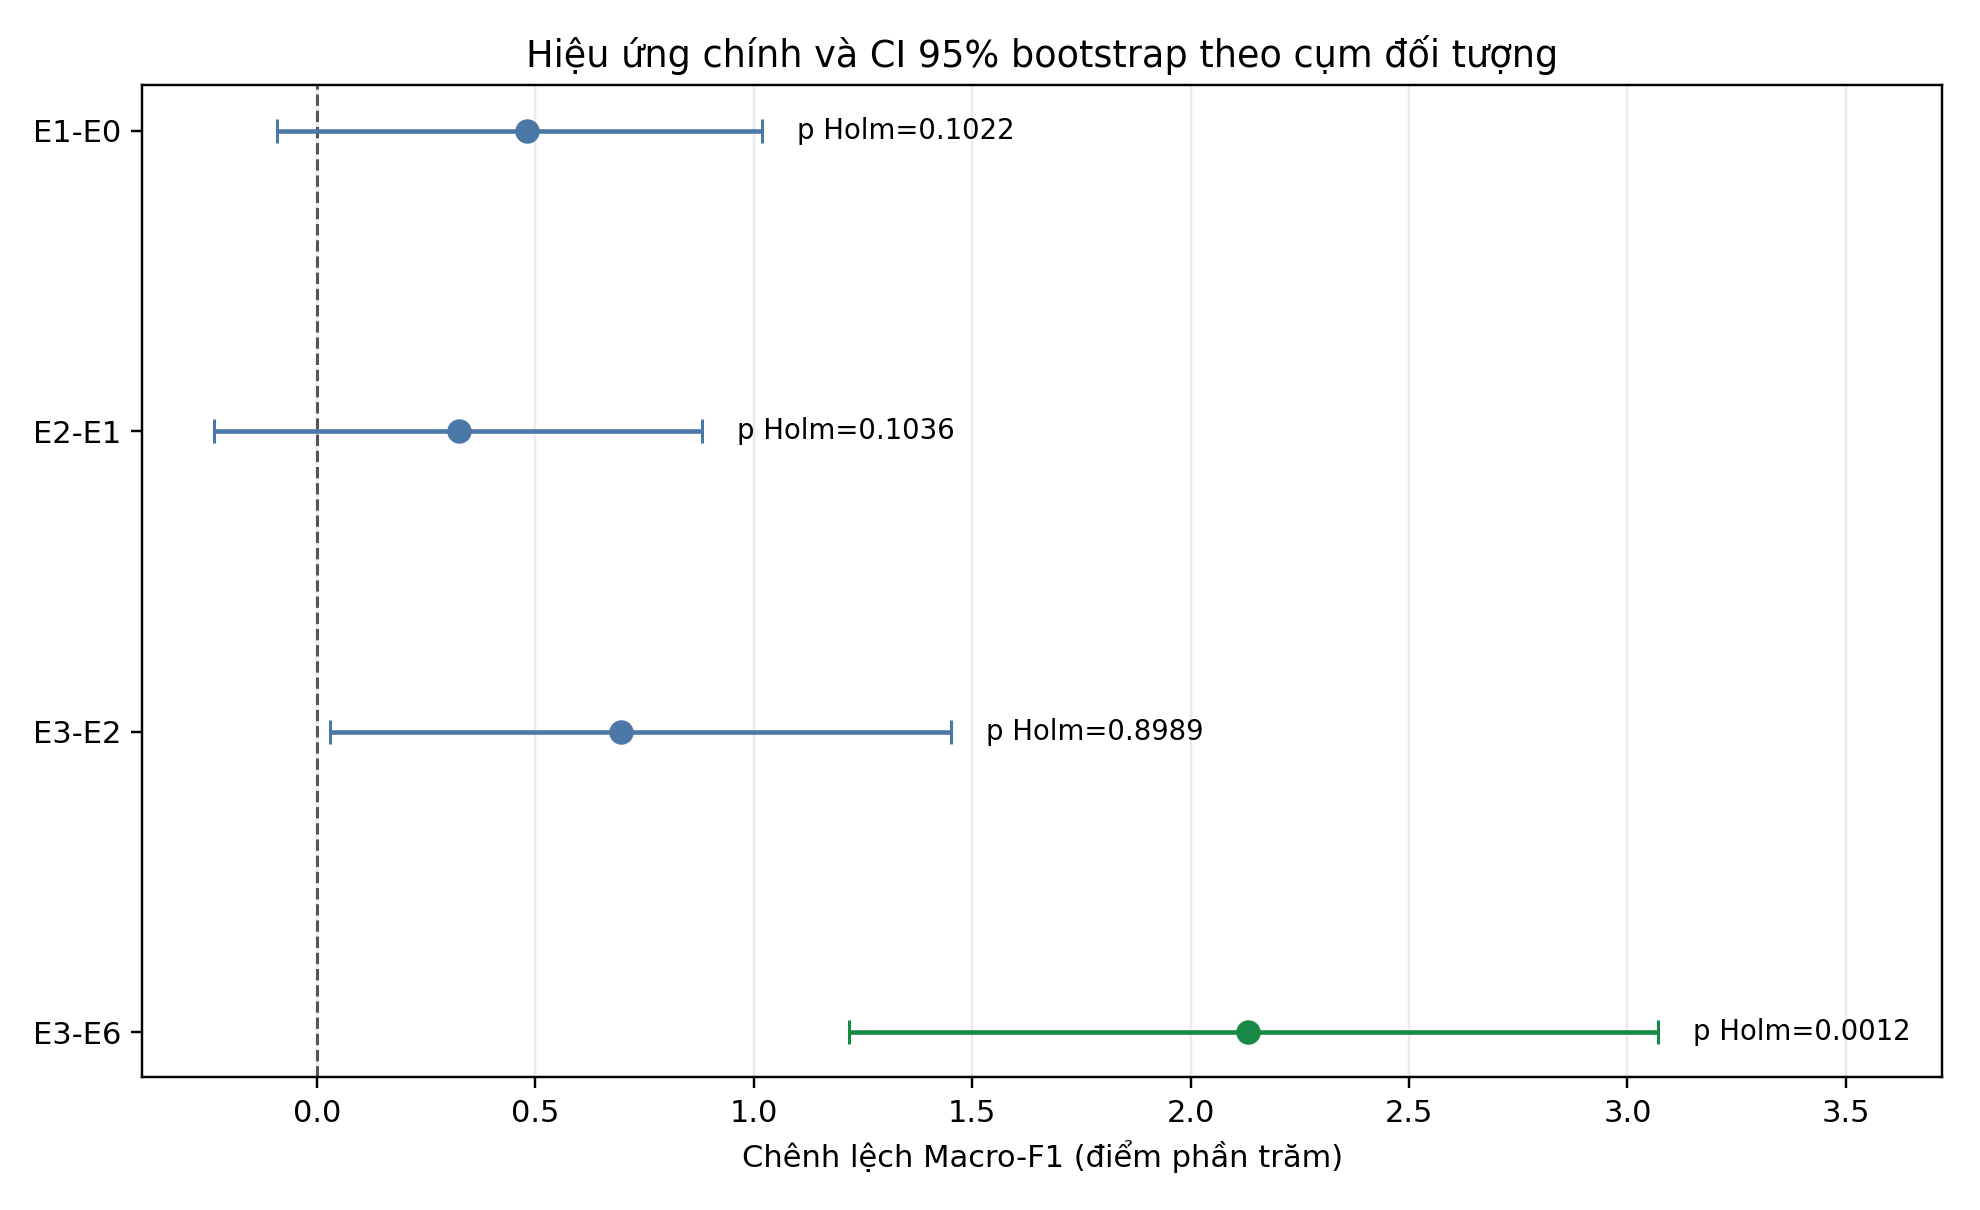
\includegraphics[width=0.95\textwidth]{../figures/gate8_primary_effects.png}
\caption{Chênh lệch \mf\ và khoảng tin cậy bootstrap cụm theo đối tượng trên Sleep-EDF.}
\label{fig:primary-effects}
\end{figure}

Đối chiếu hậu nghiệm E3--E0 cho $\Delta\mf=0,015024$, \ci\ $[0,005746;0,025871]$, Wilcoxon $p=0,012321$ và thắng/hòa/thua 49/0/29. Kết quả củng cố lợi ích của toàn bộ pipeline E3 trong chiến dịch hiện tại, bao gồm đồng thời cấu hình mô hình, tiền xử lý và lịch huấn luyện.

\subsection{Phân tích lỗi theo lớp trên Sleep-EDF}

Phân tích lớp sử dụng dự đoán ngoài fold gộp của seed 42. Bảng~\ref{tab:sleepedf-class-errors} báo cáo precision, recall, F1 của E3 và E6 cùng chênh lệch F1. Đây là thống kê mô tả trên cùng tập dự đoán kiểm tra, không phải một họ kiểm định mới.

\begin{table}[t]
\centering
\caption{Chỉ số theo lớp trên Sleep-EDF: E3 so với E6.}
\label{tab:sleepedf-class-errors}
\scriptsize
\resizebox{\textwidth}{!}{%
\begin{tabular}{lrrrrrrr}
\toprule
\textbf{Lớp} & \textbf{E3 Prec.} & \textbf{E3 Recall} & \textbf{E3 F1} & \textbf{E6 Prec.} & \textbf{E6 Recall} & \textbf{E6 F1} & \textbf{$\Delta$F1} \\
\midrule
W & 0,933784 & 0,927086 & 0,930423 & 0,939099 & 0,916911 & 0,927872 & +0,002551 \\
N1 & 0,514858 & 0,540981 & 0,527597 & 0,503248 & 0,521885 & 0,512397 & +0,015199 \\
N2 & 0,858256 & 0,844674 & 0,851411 & 0,840123 & 0,836805 & 0,838460 & +0,012950 \\
N3 & 0,807187 & 0,809725 & 0,808454 & 0,716010 & 0,777897 & 0,745672 & +0,062782 \\
REM & 0,827439 & 0,841339 & 0,834331 & 0,822702 & 0,819741 & 0,821219 & +0,013113 \\
\bottomrule
\end{tabular}}
\end{table}

N1 là lớp khó nhất của E3. Chênh lệch F1 lớn nhất nằm ở N3, trong khi các lớp còn lại cải thiện ở mức nhỏ hơn. Trong ma trận nhầm lẫn E3, các cặp sai số lớn nhất là N2$\rightarrow$N1 (5.496), N1$\rightarrow$N2 (4.867), W$\rightarrow$N1 (3.888), N1$\rightarrow$W (3.283) và N2$\rightarrow$REM (2.432). Các số đếm này chỉ mô tả cấu trúc sai số của mẫu Sleep-EDF.

\begin{table}[t]
\centering
\caption{Ma trận nhầm lẫn gộp của E3 trên Sleep-EDF.}
\label{tab:sleepedf-confusion}
\scriptsize
\begin{tabular}{lrrrrr}
\toprule
\textbf{Thật $\backslash$ Dự đoán} & \textbf{W} & \textbf{N1} & \textbf{N2} & \textbf{N3} & \textbf{REM} \\
\midrule
W & 61.133 & 3.888 & 416 & 56 & 448 \\
N1 & 3.283 & 11.643 & 4.867 & 105 & 1.624 \\
N2 & 539 & 5.496 & 58.394 & 2.271 & 2.432 \\
N3 & 30 & 45 & 2.377 & 10.558 & 29 \\
REM & 483 & 1.542 & 1.984 & 90 & 21.736 \\
\bottomrule
\end{tabular}
\end{table}

\subsection{Độ nhạy theo seed huấn luyện}

\begin{table}[t]
\centering
\caption{Macro-F1 test ngoài fold của hai seed cố định. Seed 42 là chiến dịch chính; seed 123 là lần lặp sau giao thức.}
\label{tab:multiseed-performance}
\small
\begin{tabular}{lrr}
\toprule
\textbf{Cấu hình} & \textbf{Seed 42} & \textbf{Seed 123} \\
\midrule
E0 & 0,775419 & 0,775457 \\
E1 & 0,780230 & 0,777645 \\
E2 & 0,783481 & 0,782787 \\
E3 & 0,790443 & 0,788265 \\
E4 & 0,789067 & 0,788673 \\
E6 & 0,769124 & 0,778016 \\
\bottomrule
\end{tabular}
\end{table}

\begin{table}[t]
\centering
\caption{Độ nhạy của bốn đối chiếu chính. Mỗi p-value được hiệu chỉnh Holm trong seed tương ứng; không có kiểm định gộp hai seed.}
\label{tab:multiseed-effects}
\small
\resizebox{\textwidth}{!}{%
\begin{tabular}{lrr}
\toprule
\textbf{So sánh} & \textbf{Seed 42: $\Delta$ [CI], $p_{Holm}$} & \textbf{Seed 123: $\Delta$ [CI], $p_{Holm}$} \\
\midrule
E1--E0 & 0,004811 [$-0,000915$; 0,010193], 0,1022 & 0,002188 [$-0,002870$; 0,007043], 0,9130 \\
E2--E1 & 0,003251 [$-0,002370$; 0,008808], 0,1036 & 0,005143 [$-0,000571$; 0,011292], 0,2400 \\
E3--E2 & 0,006962 [0,000305; 0,014520], 0,8989 & 0,005478 [$-0,002611$; 0,015796], 0,9130 \\
E3--E6 & 0,021319 [0,012179; 0,030698], 0,0012 & 0,010249 [0,002435; 0,017989], 0,1313 \\
\bottomrule
\end{tabular}
}
\end{table}

Cả bốn chênh lệch giữ hướng dương ở hai seed. E3--E6 là đối chiếu duy nhất có CI bootstrap hoàn toàn dương trong cả hai lần chạy, nhưng chỉ seed 42 đạt ý nghĩa Wilcoxon sau Holm. Hướng hiệu ứng vì vậy ổn định qua hai seed cố định, còn độ mạnh suy luận thì không.

\subsection{Đánh đổi độ phức tạp và tốc độ}

\begin{table}[t]
\centering
\caption{Thời gian suy luận trên Tesla V100.}
\label{tab:complexity}
\small
\begin{tabular}{lrrrrr}
\toprule
\textbf{E} & \textbf{Tham số} & \textbf{Trung vị (ms)} & \textbf{Tốc độ xử lý} & \textbf{Bộ nhớ đỉnh} & \textbf{Nhanh hơn E0} \\
\midrule
E0 & 248.630 & 13,4315 & 7.445 & 58,81 & 1,00$\times$ \\
E1 & 640.950 & 12,5111 & 7.993 & 60,31 & 1,07$\times$ \\
E2 & 1.085.578 & 3,5750 & 27.972 & 75,54 & 3,76$\times$ \\
E3 & 1.085.578 & 3,5687 & 28.021 & 75,54 & 3,76$\times$ \\
E6 & 1.085.578 & 3,5756 & 27.967 & 75,54 & 3,76$\times$ \\
\bottomrule
\end{tabular}
\end{table}

ResNet-1D--TCN có cấu trúc vận hành gọn hơn và nhanh hơn E0 khoảng 3,76 lần trong phép đo suy luận đã chuẩn hóa. Đổi lại, số tham số tăng 4,37 lần và bộ nhớ đỉnh tăng 28,4\%. Vì vậy, ưu điểm của cấu hình này nằm ở hiệu năng và tốc độ xử lý, không phải ở việc giảm quy mô mô hình.

Phép đo trên chỉ phản ánh thời gian suy luận sau khi mô hình đã được huấn luyện. Để ghi nhận chi phí tạo mô hình, Bảng~\ref{tab:training-runtime} tổng hợp thời gian thực đo của chiến dịch seed 123 trên cùng GPU Tesla V100. Các lượt được chạy tuần tự trên 10 fold; thời gian bao gồm huấn luyện, xác thực và hoàn thiện đầu ra, trong khi tập kiểm tra chưa được mở.

\begin{table}[t]
\centering
\caption{Thời gian huấn luyện và xác thực của chiến dịch seed 123.}
\label{tab:training-runtime}
\small
\begin{tabular}{lrr}
\toprule
\textbf{Cấu hình} & \textbf{Tổng 10 fold} & \textbf{Trung bình/fold} \\
\midrule
E0 --- CNN đối chứng + BiLSTM & 33 giờ 35 phút 36 giây & 3 giờ 21 phút 34 giây \\
E1 --- CNN đối chứng + TCN & 14 phút 17 giây & 1 phút 26 giây \\
E2 --- ResNet-1D + TCN & 2 giờ 44 phút 57 giây & 16 phút 30 giây \\
E3 --- ResNet-1D + TCN, xử lý chính & 3 giờ 16 phút 40 giây & 19 phút 40 giây \\
E4 --- ResNet-1D + TCN, lọc dải & 2 giờ 55 phút 56 giây & 17 phút 36 giây \\
E6 --- ResNet-1D + TCN, z-score & 2 giờ 24 phút 44 giây & 14 phút 28 giây \\
\midrule
\textbf{Toàn bộ sáu cấu hình} & \textbf{45 giờ 12 phút 10 giây} & \textbf{4 giờ 31 phút 13 giây} \\
\bottomrule
\end{tabular}
\end{table}

Trong chiến dịch này, tổng thời gian huấn luyện và xác thực của E2 thấp hơn E0 khoảng 12,2 lần; E3 thấp hơn khoảng 10,2 lần. Các tỷ lệ này mô tả toàn bộ quy trình với số epoch thực tế, quy tắc dừng sớm và lịch huấn luyện tương ứng của từng cấu hình trên cùng phần cứng.

\begin{figure}[t]
\centering
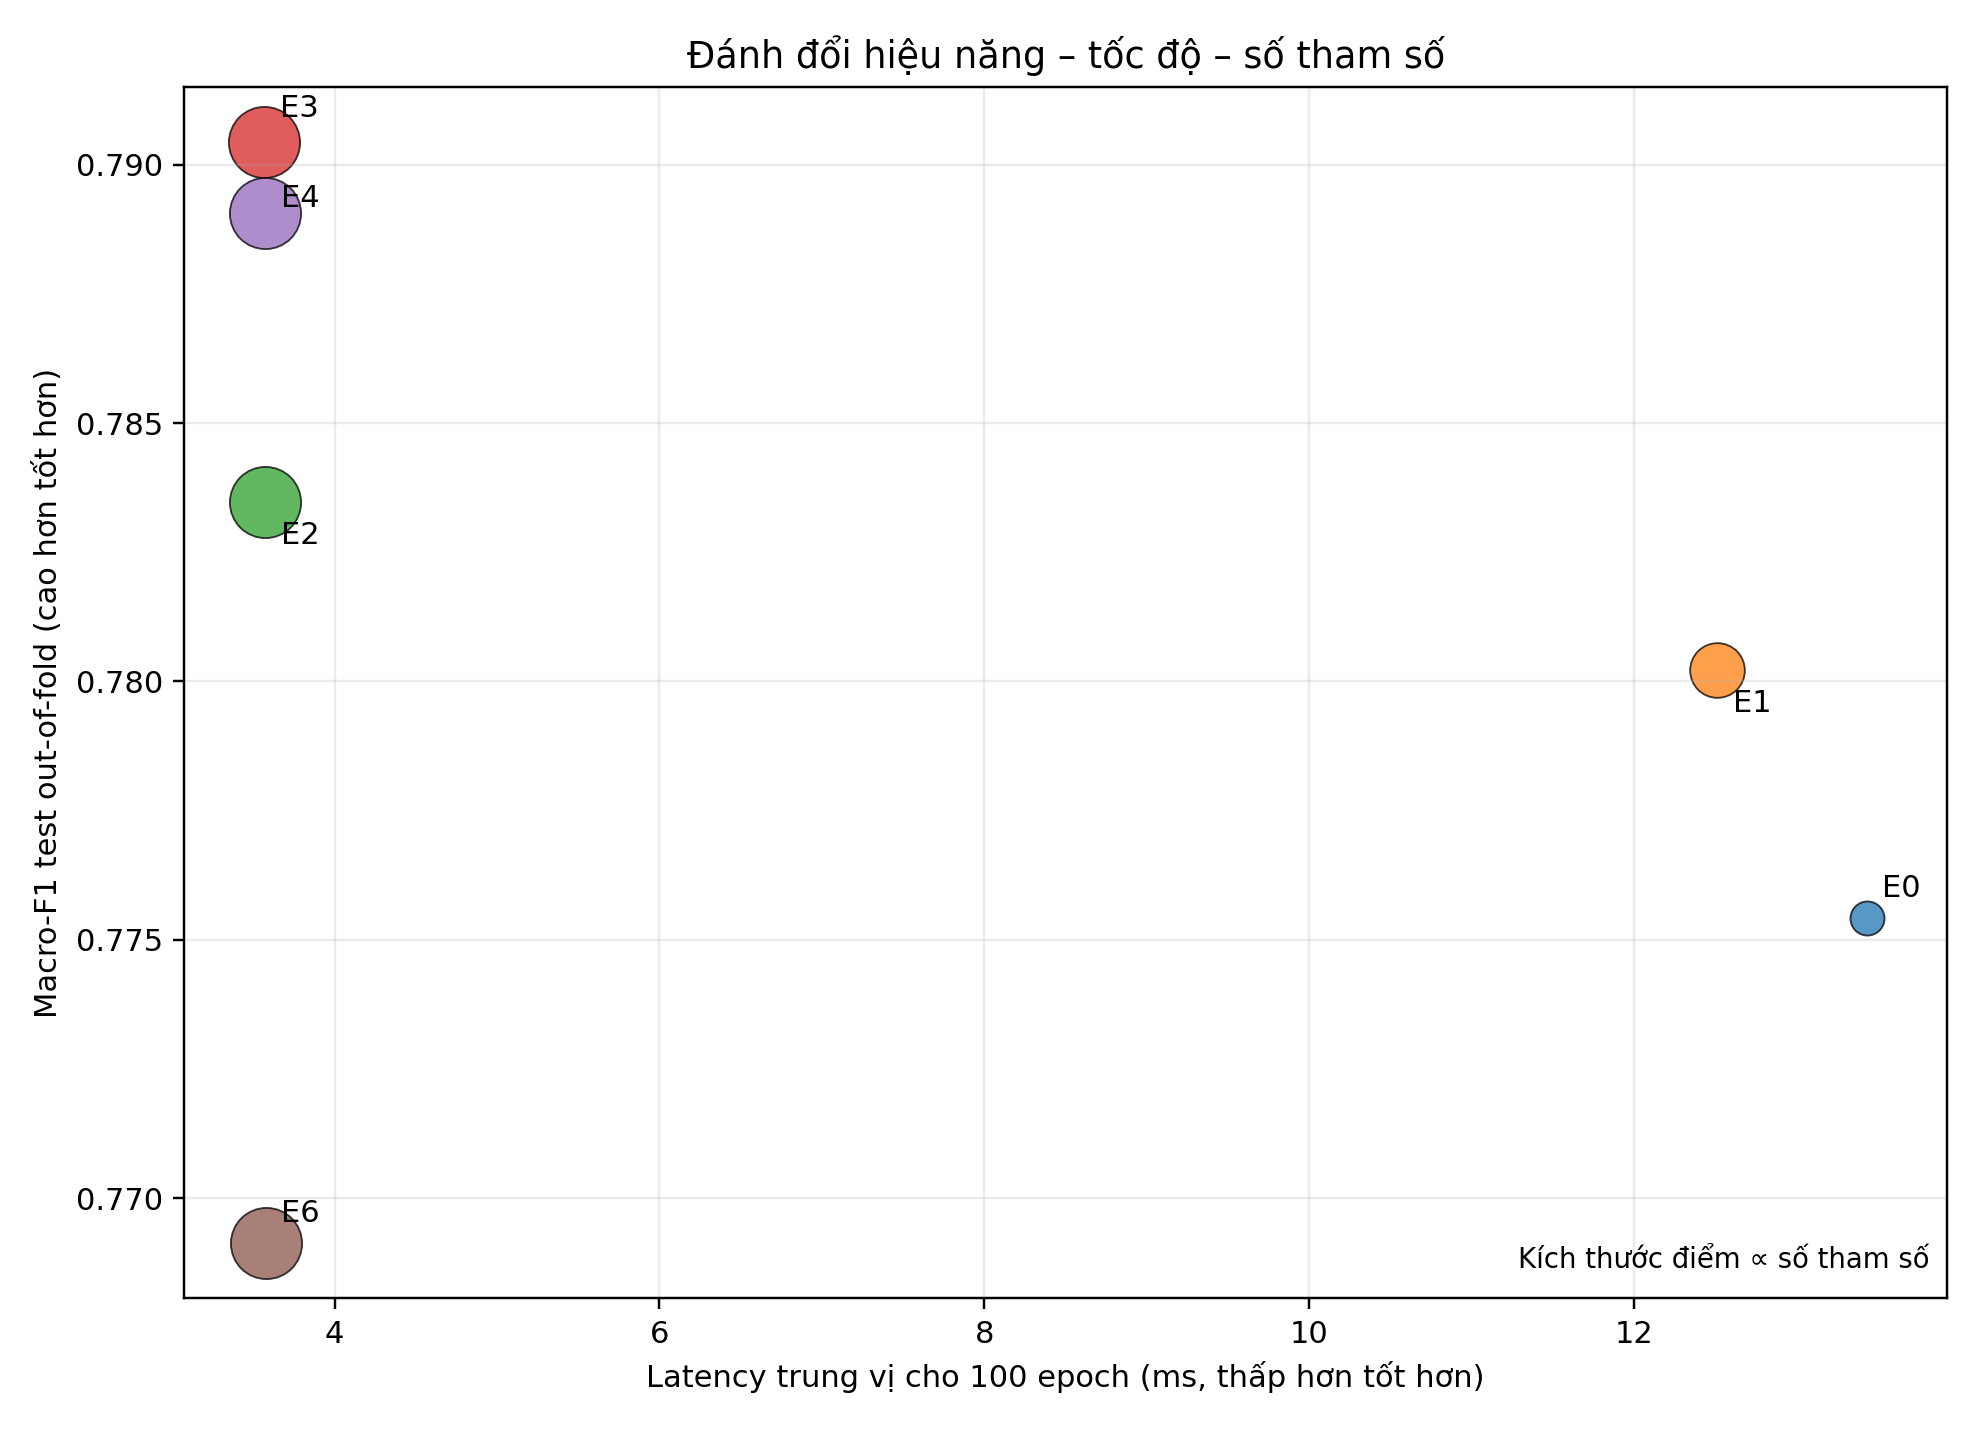
\includegraphics[width=0.88\textwidth]{../figures/gate8_performance_speed_tradeoff.png}
\caption{Đánh đổi giữa \mf, độ trễ và số tham số. Diện tích điểm tỷ lệ với số tham số.}
\label{fig:tradeoff}
\end{figure}

\subsection{Không gian đặc trưng và ablation ngữ cảnh}

Silhouette của E2 thấp hơn E1 trong toàn bộ các fold; chênh lệch E2--E1 trung bình là $-0,107851$. Kết quả không hỗ trợ giả thuyết biểu diễn ResNet tạo cụm Euclid tách lớp tốt hơn biểu diễn của mô hình CNN đối chứng, nhưng cũng không chứng minh mô hình đối chứng tốt hơn cho dự đoán chuỗi.

Phân tích loại bỏ nhóm ngữ cảnh tại vùng chuyển pha không cho thấy lợi ích tăng thêm có ý nghĩa thống kê. Kết quả này chỉ cho biết chưa quan sát được hiệu ứng trong thiết kế hiện tại; không dùng để suy ra các thành phần bị loại bỏ là vô ích hoặc tương đương với nhóm đầy đủ.

\begin{figure}[t]
\centering
\begin{subfigure}[t]{0.49\textwidth}
\centering
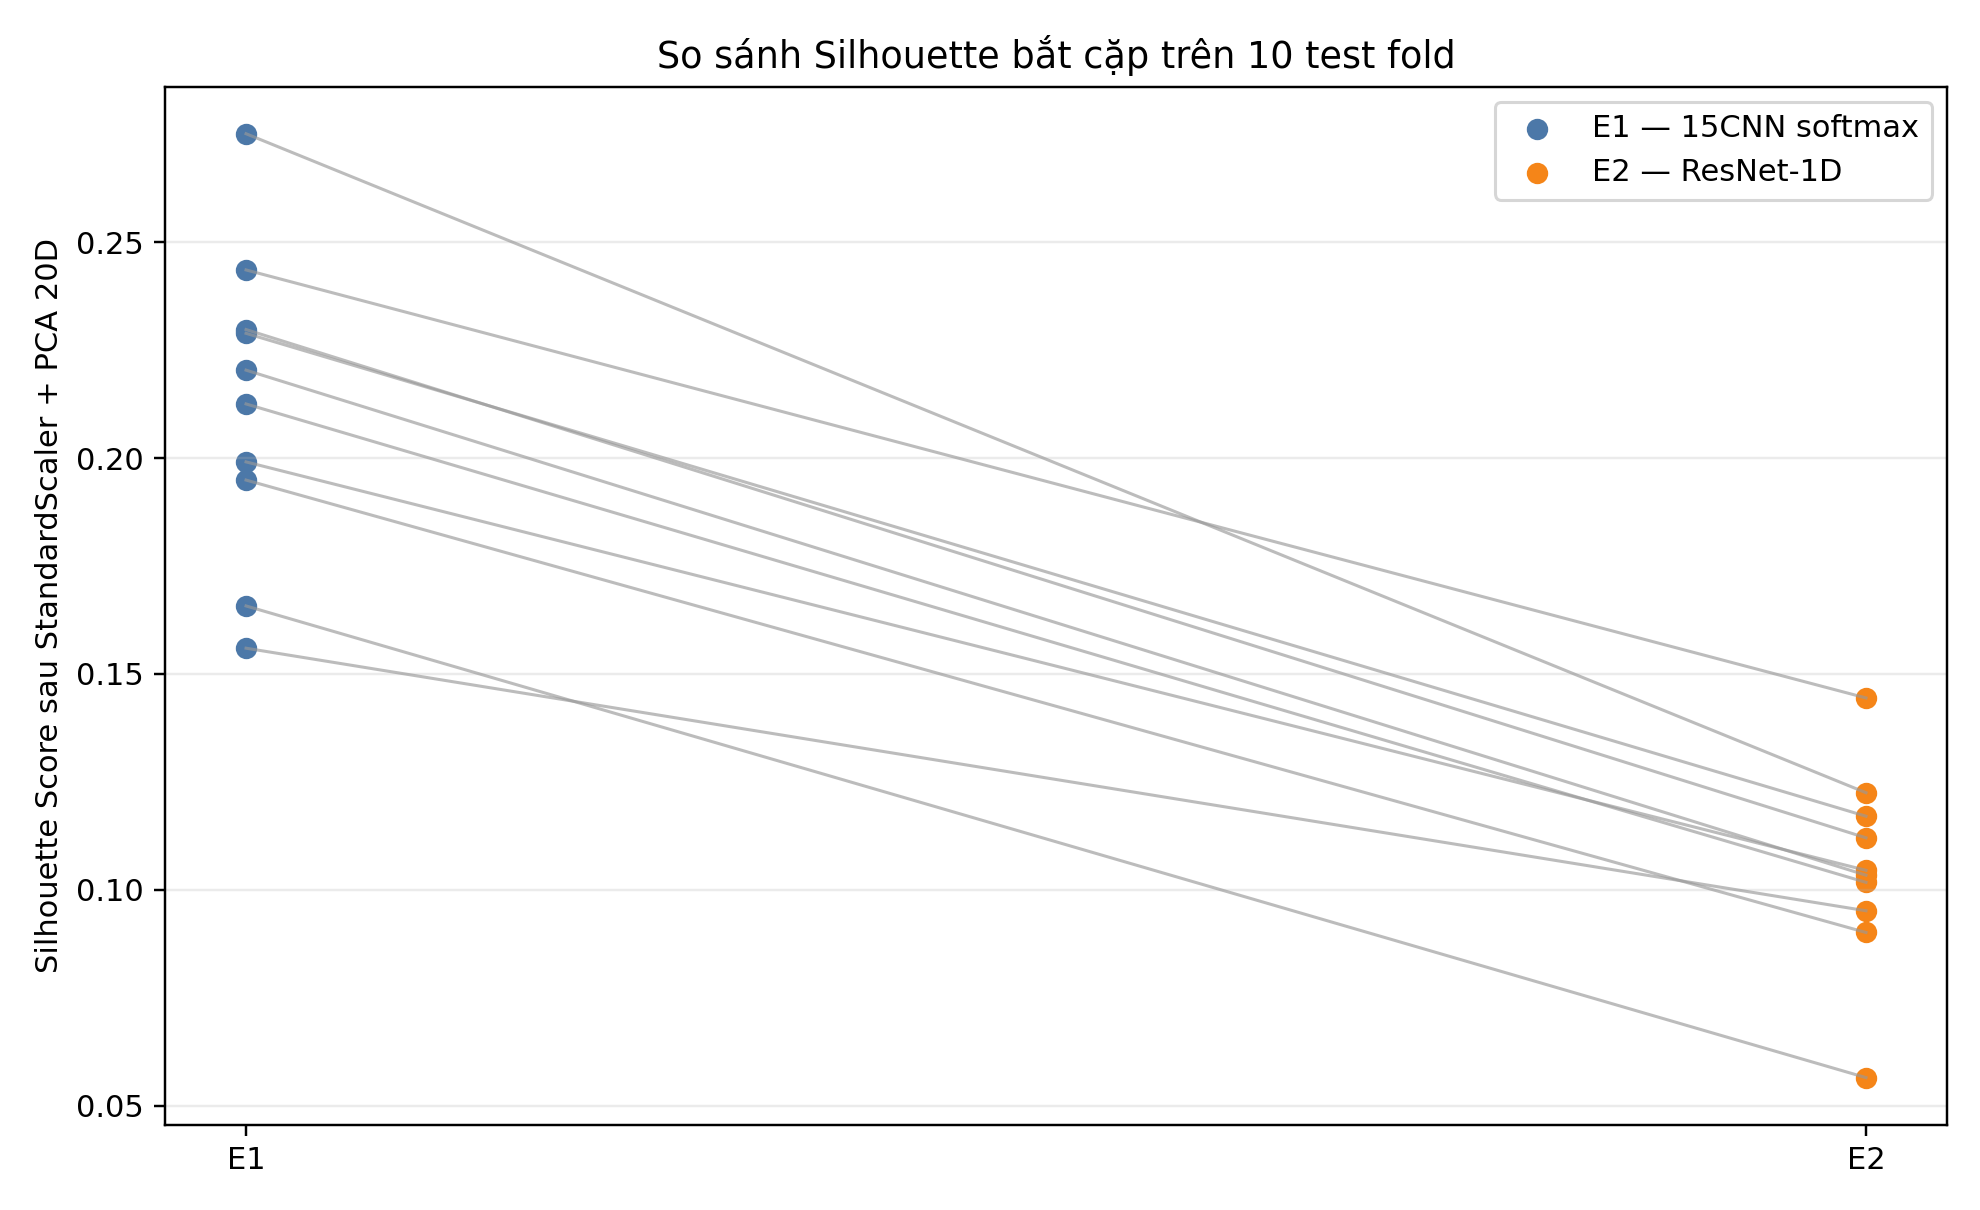
\includegraphics[width=\textwidth]{../figures/gate8_feature_silhouette.png}
\caption{Silhouette E1 và E2 theo fold.}
\end{subfigure}
\hfill
\begin{subfigure}[t]{0.49\textwidth}
\centering
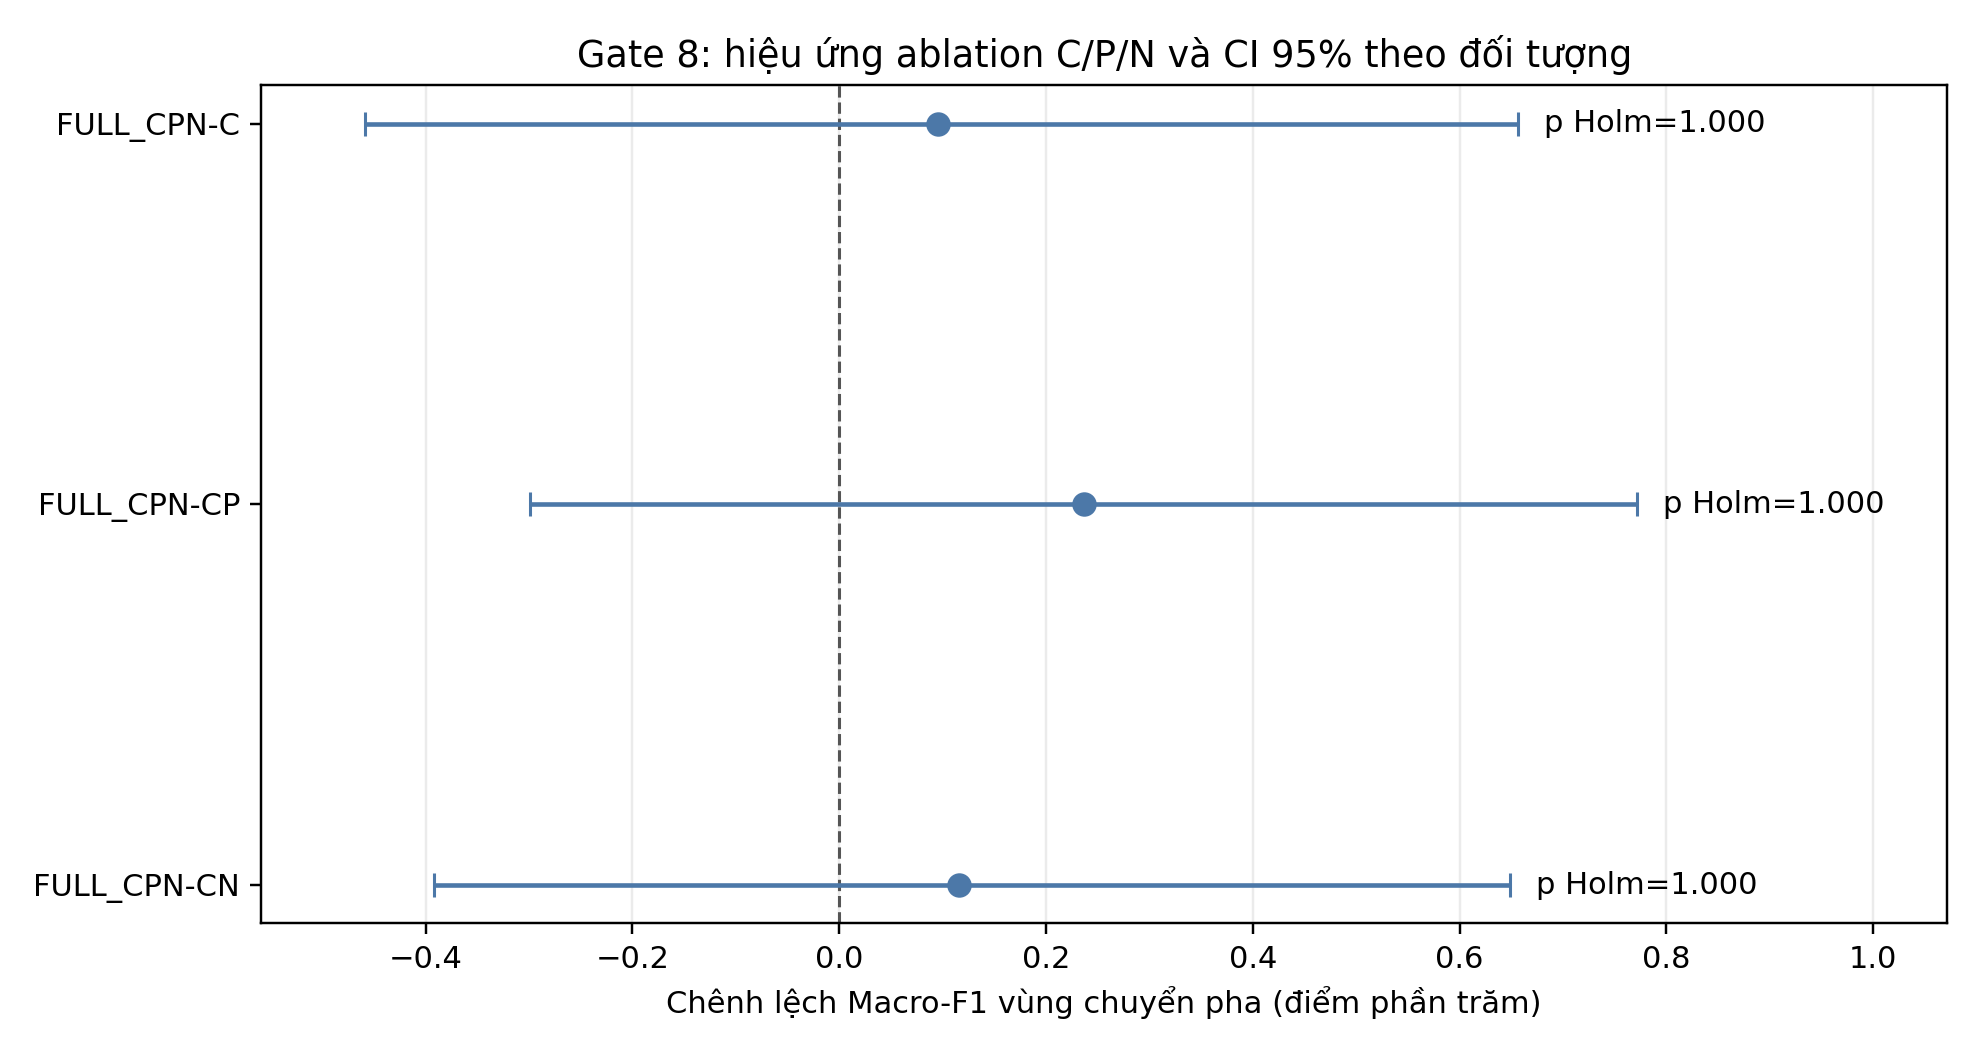
\includegraphics[width=\textwidth]{../figures/gate8_context_ablation_effects.png}
\caption{Hiệu ứng ablation C/P/N.}
\end{subfigure}
\caption{Hai phân tích hỗ trợ về biểu diễn và ngữ cảnh.}
\label{fig:supporting}
\end{figure}

\subsection{Đánh giá chuyển miền không cập nhật trọng số trên SHHS1}

\begin{table}[t]
\centering
\caption{Hiệu năng chuyển miền trên 180 đối tượng SHHS1, không cập nhật trọng số.}
\label{tab:shhs-performance}
\small
\begin{tabular}{lrrrrr}
\toprule
\textbf{E} & \textbf{\mf\ theo người} & \textbf{\mf\ gộp} & \textbf{Accuracy} & \textbf{$\kappa$} & \textbf{F1 N1} \\
\midrule
E0 & 0,5268 & 0,5761 & 0,6648 & 0,5339 & 0,2998 \\
E3 & \textbf{0,5680} & \textbf{0,6099} & \textbf{0,7016} & \textbf{0,5801} & \textbf{0,3451} \\
E6 & 0,5407 & 0,5732 & 0,6742 & 0,5408 & 0,3102 \\
\bottomrule
\end{tabular}
\end{table}

E3 cao hơn E0 0,0412 \mf\ trung bình theo đối tượng (\ci\ $[0,0314;0,0512]$, $p_{Holm}=2,65\times10^{-13}$, thắng/hòa/thua 138/0/42) và cao hơn E6 0,0274 (\ci\ $[0,0182;0,0370]$, $p_{Holm}=1,87\times10^{-8}$, 125/0/55). Các chỉ số hỗ trợ cùng hướng: so với E0, E3 tăng \mf\ gộp 0,0338, accuracy 0,0368 và $\kappa$ 0,0461. Tại vùng $\pm1$ epoch quanh chuyển pha, E3 tăng \mf\ 0,0366 so với E0 và 0,0183 so với E6.

\begin{figure}[t]
\centering
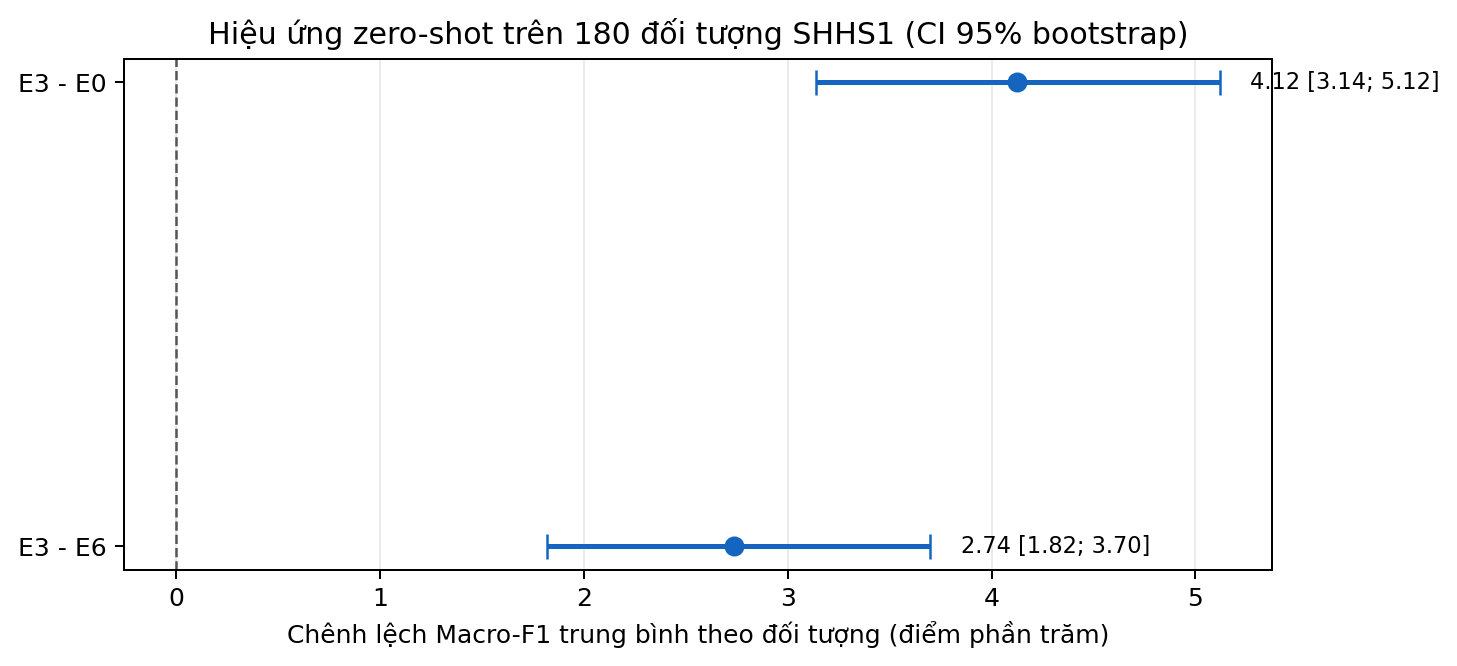
\includegraphics[width=0.88\textwidth]{../figures/shhs_zero_shot_effects.png}
\caption{Hiệu ứng chuyển miền bắt cặp theo đối tượng trên SHHS1.}
\label{fig:shhs-effects}
\end{figure}

N1 vẫn là lớp khó nhất. E3 có F1 N1 cao hơn E0, nhưng recall N1 thấp hơn (0,5437 so với 0,5841) và precision cao hơn (0,2528 so với 0,2017). Lợi ích F1 vì vậy phản ánh cân bằng precision--recall tốt hơn, không phải tăng đồng thời mọi chỉ số.

\subsection{Phân tích lỗi theo lớp trên SHHS1}

Phân tích mô tả trên 169.012 epoch hợp lệ cho thấy E3 cải thiện F1 ở cả năm lớp so với E2, với mức tăng lớn nhất ở REM và N1. Tuy vậy, recall N3 vẫn thấp và precision REM còn hạn chế, cho thấy độ bền ngoài miền vẫn phụ thuộc vào từng lớp.

\begin{table}[t]
\centering
\caption{Chỉ số theo lớp trên SHHS1: E3 so với E2.}
\label{tab:shhs-class-errors}
\scriptsize
\resizebox{\textwidth}{!}{%
\begin{tabular}{lrrrrrrr}
\toprule
\textbf{Lớp} & \textbf{E3 Prec.} & \textbf{E3 Recall} & \textbf{E3 F1} & \textbf{E2 Prec.} & \textbf{E2 Recall} & \textbf{E2 F1} & \textbf{$\Delta$F1} \\
\midrule
W & 0,882267 & 0,801395 & 0,839889 & 0,878039 & 0,727469 & 0,795694 & +0,044195 \\
N1 & 0,252822 & 0,543702 & 0,345150 & 0,236726 & 0,352756 & 0,283322 & +0,061828 \\
N2 & 0,739422 & 0,734896 & 0,737152 & 0,736197 & 0,693735 & 0,714336 & +0,022816 \\
N3 & 0,944044 & 0,258178 & 0,405468 & 0,965898 & 0,249627 & 0,396725 & +0,008743 \\
REM & 0,605237 & 0,893923 & 0,721785 & 0,488616 & 0,944976 & 0,644158 & +0,077626 \\
\bottomrule
\end{tabular}}
\end{table}

Trong ma trận nhầm lẫn E3, các cặp sai số lớn nhất là N3$\rightarrow$N2 (16.674), N2$\rightarrow$REM (11.605), N2$\rightarrow$N1 (5.947), W$\rightarrow$N1 (4.481) và N2$\rightarrow$W (2.348). Đối chiếu cùng mẫu cho thấy E0 cũng gán 16.480/22.806 epoch N3 thành N2, tương ứng 72,3\%, và có recall N3 0,2610 so với 0,2582 của E3. Vì vậy, lỗi N3$\rightarrow$N2 tái diễn ở cả hai họ kiến trúc: E3 cải thiện hiệu năng tổng thể và có precision N3 cao hơn (0,9440 so với 0,9007), nhưng chưa khắc phục việc bỏ sót N3.

Trong kiểm tra hậu nghiệm dùng cùng định nghĩa vùng lân cận thay đổi nhãn, \mf\ của E0/E3 tại vùng lân cận so với vùng ổn định là 0,6179/0,6321 so với 0,8175/0,8346 trên Sleep-EDF, và 0,4323/0,4689 so với 0,5959/0,6220 trên SHHS1. Recall N3 tương ứng là 0,6121/0,6326 so với 0,9216/0,9316 trên Sleep-EDF, nhưng chỉ 0,0633/0,0733 so với 0,4008/0,3900 trên SHHS1. Kết quả cùng hướng khi chỉ giữ các thay đổi nhãn có ít nhất ba epoch liên tiếp cùng nhãn ở mỗi phía. Thiếu N3 vì vậy không giới hạn ở vùng ranh giới và vẫn hiện diện rõ trong các vùng nhãn ổn định của SHHS1.

\begin{table}[t]
\centering
\caption{Thiếu N3 tái diễn trên SHHS1 seed 42; mẫu gồm 22.806 epoch N3 thật.}
\label{tab:shhs-n3-shared}
\small
\begin{tabular}{lrrrr}
\toprule
\textbf{Cấu hình} & \textbf{Precision N3} & \textbf{Recall N3} & \textbf{F1 N3} & \textbf{N3$\rightarrow$N2} \\
\midrule
E0 & 0,9007 & 0,2610 & 0,4048 & 72,3\% \\
E3 & 0,9440 & 0,2582 & 0,4055 & 73,1\% \\
E6 & 0,9052 & 0,2005 & 0,3283 & 77,9\% \\
\bottomrule
\end{tabular}
\end{table}

Pipeline z-score E6 đạt recall N3 0,2005, thấp hơn 0,2582 của E3, và tỷ lệ N3 thành N2 là 77,9\% (Bảng~\ref{tab:shhs-n3-shared}). Tại vùng lân cận thay đổi nhãn, recall N3 của E6/E3 là 0,0721/0,0733. Kết quả cho thấy pipeline z-score đã thử không khắc phục thiếu N3; do mỗi pipeline được huấn luyện riêng, nó không cô lập vai trò biên độ hoặc loại trừ các phương pháp thích nghi không nhãn khác.

\begin{table}[t]
\centering
\caption{Ma trận nhầm lẫn gộp của E3 trên SHHS1.}
\label{tab:shhs-confusion}
\scriptsize
\begin{tabular}{lrrrrr}
\toprule
\textbf{Thật $\backslash$ Dự đoán} & \textbf{W} & \textbf{N1} & \textbf{N2} & \textbf{N3} & \textbf{REM} \\
\midrule
W & 29.638 & 4.481 & 1.171 & 21 & 1.672 \\
N1 & 874 & 3.807 & 601 & 3 & 1.717 \\
N2 & 2.348 & 5.947 & 56.063 & 324 & 11.605 \\
N3 & 78 & 39 & 16.674 & 5.888 & 127 \\
REM & 655 & 784 & 1.311 & 1 & 23.183 \\
\bottomrule
\end{tabular}
\end{table}

\subsection{Phân tích thành phần ngoài miền}

E1--E0 trên SHHS đạt $+0,00651$ \mf\ theo đối tượng, \ci\ $[0,00192;0,01087]$, $p_{Holm}=0,00325$ và thắng/hòa/thua 108/0/72. Đây là lợi ích nhỏ của cấu hình TCN cùng lịch huấn luyện tương ứng khi giữ bộ trích đặc trưng E0. E2--E1 đạt $-0,01280$, \ci\ $[-0,02209;-0,00350]$, $p_{Holm}=0,01005$ và 80/0/100; gói ResNet-1D 128 chiều chỉ dùng epoch hiện tại không vượt gói CNN C/P/N 75 chiều trên tín hiệu SHHS chưa lọc dải. Vì toàn bộ gói đặc trưng/ngữ cảnh thay đổi, chênh lệch này không thể quy riêng cho encoder.

Đối chiếu hậu nghiệm E3--E2, cùng họ ResNet-1D--TCN và lịch huấn luyện nhưng khác chế độ tiền xử lý, cho $+0,04750$ \mf\ theo đối tượng, \ci\ $[0,03724;0,05792]$, Wilcoxon $p=2,35\times10^{-17}$ và thắng/hòa/thua 147/0/33. F1 N1 tăng 0,06183 và \mf\ vùng chuyển pha tăng 0,04700. Đây là chênh lệch Macro-F1 trung bình theo đối tượng lớn nhất trong các đối chiếu cấu hình SHHS1 được báo cáo.

Một phân tích mở rộng sử dụng checkpoint seed 123 của cả năm cấu hình để đánh giá E4, chỉ sử dụng lọc dải, trên cùng mẫu SHHS1. E4 đạt \mf\ theo đối tượng 0,5732, \mf\ gộp 0,6147, accuracy 0,7064, $\kappa=0,5869$ và F1 N1 0,3492. So với E2 cùng seed, chênh lệch \mf\ theo đối tượng là $+0,03232$, CI 95\% $[0,02365;0,04104]$, Wilcoxon--Holm $p=7,40\times10^{-13}$ và thắng/hòa/thua 135/1/44. E4 cũng cao hơn E3 cùng seed 0,00982, CI $[0,00730;0,01250]$ và $p_{Holm}=1,89\times10^{-10}$. Các đối chiếu này được xem là bằng chứng thứ cấp vì thực hiện sau khi mẫu SHHS1 đã được mở.

\section{Thảo luận}

\subsection{Hiệu năng pipeline và đánh đổi vận hành}

E3 kết hợp được hiệu năng dự báo cao với lợi ích vận hành rõ rệt. Ở seed 42, cấu hình này dẫn đầu các chỉ số gộp trên Sleep-EDF và vượt E0/E6 trong hai đối chiếu chính trên SHHS1. ResNet-1D--TCN cũng tăng tốc suy luận khoảng 3,76 lần, dù số tham số và bộ nhớ GPU cao hơn. Khi huấn luyện, E2 và E3 hoàn tất 10 fold seed 123 trong khoảng 2,75 và 3,28 giờ, so với hơn 33,5 giờ của E0. Đây là đánh đổi có ý nghĩa cho vòng phát triển và kiểm tra pipeline, không phải một mô hình nhẹ hơn trên mọi phương diện.

Các phép thay cấu hình riêng cần được đọc khác với lợi ích của toàn pipeline. E1--E0 thay BiLSTM bằng TCN cùng learning rate, batch size và dừng sớm khác; E2--E1 thay gói C/P/N, encoder, số chiều và cách huấn luyện/chọn encoder. Hai chênh lệch Sleep-EDF nhỏ chưa đạt ý nghĩa Wilcoxon sau Holm. Trên SHHS, E1--E0 dương nhưng nhỏ, còn E2--E1 âm. Do đó, kết quả đo được thuộc về những cấu hình đã triển khai, không xác lập TCN hoặc ResNet tự thân vượt trội.

Với E3--E2 Sleep-EDF, CI bootstrap gộp dương trong khi Wilcoxon theo người không đạt ý nghĩa. Macro-F1 từ tổng ma trận nhầm lẫn không phải trung bình có trọng số của Macro-F1 từng người; hai phép phân tích không thiết lập lợi ích đồng đều và không tự xác định nhóm người tạo ra phần tăng gộp. E3--E6 nhất quán hơn về hướng: CI gộp dương ở cả hai seed, nhưng độ lớn giảm từ 0,0213 xuống 0,0102 và seed 123 không giữ ý nghĩa sau Holm. E4 cũng nhỉnh hơn E3 ở seed 123, nên thứ hạng cao nhất của E3 chỉ áp dụng cho chiến dịch chính seed 42.

\subsection{Tiền xử lý và thiếu N3 khi chuyển cohort}

Trong đối chiếu hậu nghiệm SHHS1 đã quan sát, E3--E2 có chênh lệch Macro-F1 trung bình theo người lớn hơn E1--E0 và E2--E1. Phần mở rộng seed 123 cho thấy E4 chỉ lọc dải cao hơn cả E2 và E3 cùng seed. Các kết quả làm nổi bật vai trò đáng kể của cấu hình tiền xử lý trong mẫu này. Tuy nhiên, các đối chiếu ở cấp cấu hình không tách được đóng góp của từng thao tác tiền xử lý. Kiểm toán Sleep-EDF xác nhận E4/E5 trùng từng bit trên 153 bản ghi; kiểm toán SHHS riêng cũng ghi nhận không có mẫu vượt ngưỡng giới hạn trong 200 bản ghi đã xử lý.

Lợi ích tổng thể của E3 không giải quyết được nhận diện N3 so với E0. Cả hai mô hình gán hơn 72\% N3 thành N2; thiếu hụt vẫn hiện diện ngay trong vùng nhãn ổn định của SHHS1. E6 dùng trung bình và độ lệch chuẩn toàn bản ghi đích không nhãn nhưng không khắc phục được lỗi này. Đây là kết luận về pipeline z-score đã thử, không phải bằng chứng loại trừ biên độ, montage hoặc mọi phương pháp thích nghi không nhãn. Tỷ lệ dự đoán N3 thấp mô tả tần suất phát lớp, không đo calibration xác suất.

Oracle sửa N3$\rightarrow$N2 trong ma trận E3 nâng Macro-F1 SHHS1 từ 0,6099 lên 0,7444, tương ứng 74,5\% chênh lệch điểm quan sát với Sleep-EDF. Con số này định lượng quy mô một kênh lỗi, không dự báo hiệu năng thuật toán thực tế. EDF dùng dự đoán ngoài fold, còn SHHS dùng ensemble mười mô hình; phân bố lớp và thành phần cohort cũng khác. Vì vậy, đây không phải phần mất mát nhân quả do dịch chuyển miền có thể được phục hồi bằng một biện pháp đã xác nhận.

\subsection{Giá trị của phân tích hỗ trợ và giới hạn}

Silhouette E2 thấp hơn E1 chỉ cho thấy các cụm Euclid kém tách biệt hơn trong pipeline phân tích đã dùng, không chứng minh biểu diễn E2 kém hữu ích cho dự đoán chuỗi. Ablation huấn luyện lại TCN chưa phát hiện lợi ích tăng thêm có ý nghĩa của các nhóm P/N; kết quả không thiết lập tương đương hoặc phủ định ngữ cảnh thời gian nói chung.

Nghiên cứu gồm hai seed cố định và một hướng chuyển tới mẫu 180 người SHHS1. Các phân tích thành phần và vùng nhãn hậu nghiệm không phải xác nhận độc lập. Nghiên cứu không thực hiện phân tích hiệu năng phân tầng theo giới tính hoặc giới (sex/gender), nên chưa đánh giá được mức độ nhất quán của các kết quả giữa các nhóm này. Các cohort khác đồng thời về quần thể, montage, thiết bị và thực hành chấm, nên nghiên cứu định vị lỗi mà chưa xác định nguyên nhân. Mô hình hai chiều/không nhân quả và lọc tiến--lùi chỉ phù hợp với đánh giá ngoại tuyến; thời gian forward không phải độ trễ ra quyết định trực tuyến.

Một kiểm chứng tiếp theo có thể lặp lại mẫu lỗi trên cohort chưa xem hoặc trên đối chứng mạnh dưới cùng giao thức. Nếu đánh giá biện pháp khắc phục N3, cần tách tập thích nghi/validation khỏi test và báo đồng thời recall, precision, false-positive N3, ảnh hưởng lên N2 và hiệu năng ở cả vùng lân cận lẫn vùng ổn định. Dữ liệu hiện tại chưa chứng minh chiến lược thu nhãn nào tối ưu, cũng chưa so sánh hiệu quả của calibration hoặc fine-tuning.

\section{Kết luận}

Nghiên cứu kết nối ba kết quả: hiệu năng của các cấu hình pipeline dưới cùng phép chia theo người, đánh đổi vận hành được định lượng và lỗi chuyển cohort theo lớp. E3 đạt Macro-F1 ngoài fold 0,7904 ở Sleep-EDF seed 42 và vượt E0/E6 trong các đối chiếu SHHS1 chính đã khóa. ResNet-1D--TCN đem lại mức tăng tốc suy luận 3,76 lần và thời gian huấn luyện/xác thực ngắn hơn đáng kể trong chiến dịch đã đo, với chi phí tham số và bộ nhớ cao hơn. Các lợi ích này thuộc về cấu hình và lịch huấn luyện tương ứng, không phải ưu thế kiến trúc riêng lẻ.

Trên SHHS1, E0/E3 cùng gán hơn 72\% N3 thành N2 dù E3 có điểm tổng thể cao hơn; pipeline z-score E6 cũng không khắc phục thiếu N3. Các đối chiếu hậu nghiệm về tiền xử lý và quy mô kênh lỗi N3 cung cấp mục tiêu cụ thể cho bước kiểm chứng tiếp. Đóng góp của nghiên cứu nằm ở bằng chứng pipeline, lợi ích vận hành và chẩn đoán chuyển cohort có truy nguyên, chưa phải một cơ chế sinh lý hoặc phương pháp thích nghi đã được xác nhận.

\subsection*{Khả năng tái lập và tính sẵn có dữ liệu}

Mã nguồn, giao thức, phép chia và các tổng hợp kết quả được lưu trong kho dự án công khai tại \url{https://github.com/quanuiter/SleepTCN}. Snapshot lịch sử \texttt{configs/shhs\_zero\_shot\_v1.json} khớp hash protocol ghi trong run manifest SHHS gốc; hồ sơ mở rộng sau chạy được giữ riêng. Việc khớp hash xác nhận danh tính artifact, không thay thế tái huấn luyện hoặc tái sinh dự đoán độc lập. Sleep-EDF Expanded có thể truy cập công khai qua PhysioNet (\url{https://physionet.org/content/sleep-edfx/1.0.0/}); quyền truy cập Sleep Heart Health Study được quản lý qua NSRR (\url{https://sleepdata.org/datasets/shhs/pages}) và tác giả xác nhận đã xin được quyền truy cập cho phân tích này. Kho công khai và bộ bài nộp chỉ chứa mã nguồn, giao thức, phép chia và các tổng hợp kết quả; không chứa dữ liệu cấp người tham gia SHHS, mã định danh hoặc dự đoán cấp người tham gia.

\subsection*{Đạo đức và quyền sử dụng dữ liệu}

Phân tích sử dụng dữ liệu nghiên cứu sẵn có và không tuyển người tham gia mới. Tác giả xác nhận đã xin được quyền truy cập SHHS qua NSRR cho phân tích này; theo xác nhận của tác giả, phân tích thứ cấp dữ liệu đã khử định danh không cần xét duyệt đạo đức tại đơn vị áp dụng. Báo cáo không nêu mã phê duyệt.

\subsection*{Tài trợ}

Nghiên cứu nhận khoảng 6.000.000 VND hỗ trợ sinh viên từ Trường Đại học Công nghệ Thông tin,
Đại học Quốc gia Thành phố Hồ Chí Minh.

\subsection*{Lời cảm ơn}

Nghiên cứu sử dụng Sleep-EDF Expanded do PhysioNet phân phối và dữ liệu Sleep Heart Health Study qua National Sleep Research Resource. Sleep Heart Health Study được hỗ trợ bởi các thỏa thuận hợp tác của National Heart, Lung, and Blood Institute: U01HL53916, U01HL53931, U01HL53934, U01HL53937, U01HL64360, U01HL53938, U01HL53940, U01HL53941 và U01HL63463. National Sleep Research Resource được hỗ trợ bởi National Heart, Lung, and Blood Institute (R24 HL114473 và 75N92019R002). Các tác giả trân trọng cảm ơn Nguyễn Hồ Duy Trí đã hướng dẫn học thuật, định hướng đề tài nghiên cứu và góp ý xây dựng cho các phiên bản trước của bản thảo.

\subsection*{Đóng góp của tác giả (CRediT)}

Ngô Nhật Quân là tác giả đứng đầu và tác giả liên hệ; email: \texttt{23521258@gm.uit.edu.vn}. Phạm Thái Sơn là đồng tác giả thứ hai. Hai tác giả đã đọc và duyệt bản thảo cuối. Ngô Nhật Quân: Conceptualization, Methodology, Software, Data curation, Formal analysis, Investigation, Visualization, Writing -- original draft, Writing -- review and editing. Phạm Thái Sơn: Validation, Investigation, Visualization, Writing -- review and editing.

\subsection*{Tuyên bố xung đột lợi ích}

Hai tác giả tuyên bố không có xung đột lợi ích.

\subsection*{Sử dụng công cụ AI trong chuẩn bị bản thảo}

OpenAI Codex hỗ trợ chỉnh sửa câu chữ, tổ chức nội dung, đối chiếu báo cáo với code/artifact, viết mã dựng các biểu đồ có thể tái lập từ các tổng hợp số liệu đã lưu và soạn sơ đồ quy trình xử lý nguyên bản bằng TikZ cho bản thảo tiếng Anh. Sơ đồ này chỉ minh họa luồng xử lý và mô hình, không mô tả các dạng sóng đo được. Các hỗ trợ này không huấn luyện thêm mô hình hoặc tạo dữ liệu thực nghiệm mới. Tác giả xác nhận không dùng công cụ AI nào khác cho việc chuẩn bị bản thảo. Hai tác giả đã đọc và duyệt bản cuối; trách nhiệm đối với nội dung thuộc về các tác giả.

\renewcommand{\refname}{Tài liệu tham khảo}
\begingroup
\scriptsize
\bibliographystyle{ieeetr}
\bibliography{references}
\endgroup

\end{document}
